
\section{Statics}
\subsection{Equilibrium of rigid bodies}
\begin{definition}
    {The 3 equations of equilibrium}
    A rigid body is in equilibrium if:
    \[\sum F_x=0,\quad\sum F_y=0,\quad\sum M_O=0\]
    Where $O$ is any point.
\end{definition}
\begin{definition}
    {Static equilibrium}
    A system is in \textbf{static equilibrium} if it experiences no acceleration when loads are applied to it.
\end{definition}
\begin{knBox}
    {Free body diagrams (FBD)}
    Free body diagrams are diagrams that show all the forces acting on a body. They are useful in determining the forces that cause the body to be in equilibrium.
\end{knBox}
\begin{definition}
    {Static systems}
    A static system:
    \begin{enumerate}
        \item Must be in equilibrium
        \item Does not experience any acceleration
        \item Can have mechanisms that doesn't undergo movements
    \end{enumerate}
\end{definition}

\subsection{Members}
A member is a \emph{straight} and \emph{long} structural element that is subjected to axial forces. The following are the types of members:


\subsection{Static systems}
\begin{definition}
    {Supports and reaction forces}
    Each support will restrict the movement of the rigid body in a certain way. If a certain degree of freedom is restricted, a reaction force will be present to counteract the force that would have caused the movement.
    \begin{table}[H]
        \begin{tabular}{lll}
            \textbf{Support type} & \textbf{Restricted movement and reaction forces} & \textbf{Shape} \\ \hline
            Fixed                 & x, y, r (moment)                                 & Flat           \\ \arrayrulecolor{lightgray}\hline
            Pinned                & x, y                                             & Triangle       \\ \arrayrulecolor{lightgray}\hline
            Roller                & y                                                & Circle         \\ \arrayrulecolor{lightgray}\hline
        \end{tabular}
    \end{table}
\end{definition}
\begin{definition}
    {Stable structures}
    A structure is said \emph{stable} if all members remain in place under any loading conditions. (No mechanisms)
\end{definition}

\begin{definition}
    {Static conditions of a system}
    A system's state of equilibrium can be determined by the number of restraints present:
    \begin{enumerate}
        \item Insufficient restraints $\to$ \textbf{non-static system}
        \item Sufficient restraints $\to$ \textbf{static system}
    \end{enumerate}
    A static system is said to be \textbf{statically indeterminate} if the number of unknowns is larger than the number of equations of equilibrium.
\end{definition}
\begin{theorem}
    {Degree of indeterminacy (Trusses)}
    \[I=m+r-2j\]
    Where $m$ is the number of members, $r$ is the number of reaction forces, $j$ is the number of internal hinges (circles).
\end{theorem}
\begin{theorem}
    {Degree of indeterminacy (Frames)}
    \[I=3m+r-3n-j\]
    \begin{enumerate}
        \item $m$ is the number of members (intersecting beams are separate)
        \item $r$ is the number of reaction forces
        \item $n$ is the number of nodes (all ends and intersections)
        \item $j$ is the number of internal hinges (circles)
    \end{enumerate}
\end{theorem}

\subsection{Loading}
\begin{knBox}
    {Types of loading}
    \begin{enumerate}
        \item \textbf{Concentrated load} is a force applied at a single point. ($N$)
        \item \textbf{Distributed load} is a force applied over a length. ($N/m$)
    \end{enumerate}
\end{knBox}
\begin{theorem}
    {Distributed load}
    A \emph{distributed load} $(w)$ is a force that is distributed over a length $(l)$, that has the unit $N/m$.

    The \textbf{resultant force} is the supposed area of the load. To consider the \textbf{moment} by a distributed load, we can treat the load as a \emph{single force} acting at the \textbf{centroid} of the load.
    \begin{itemize}
        \item Unifrom $\to$ $F=wl\quad @\frac{1}{2}l$
        \item Triangular $\to$ $F=\frac{1}{2}wl\quad @ \frac{1}{3}l$  (from the base of the load)
    \end{itemize}
\end{theorem}

\section{Structural analysis}
\subsection{Pin-joined trusses}
A \textbf{truss} is a structure that consists of \emph{straight members} connected at their ends by \emph{pin joints}.

A triangular truss is a statically determinate structure, but a quadrangular truss is not.
\begin{center}
    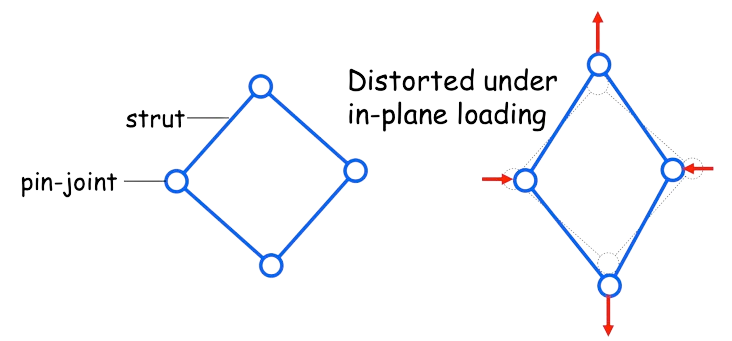
\includegraphics[width=0.45\textwidth]{./img/quadtruss.png}
    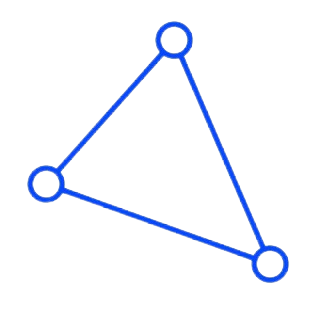
\includegraphics[width=0.2\textwidth]{./img/tritruss.png}
\end{center}
\begin{theorem}
    {Zero-force members}
    The following are zero-force members given that \textbf{no external load or support reaction is applied to the joint}.
    \begin{itemize}
        \item \textbf{2 non-collinear members} of a two-member-joint
        \item \textbf{3rd member} of a three-member-joint, where the other two are collinear.
    \end{itemize}
    Additionally, members that provide \textbf{no structural support against the applied load} are also considered to be zero-force members.

    Removing zero-force members allows us to simplify a truss structure.
    \tcblower
    \begin{center}
        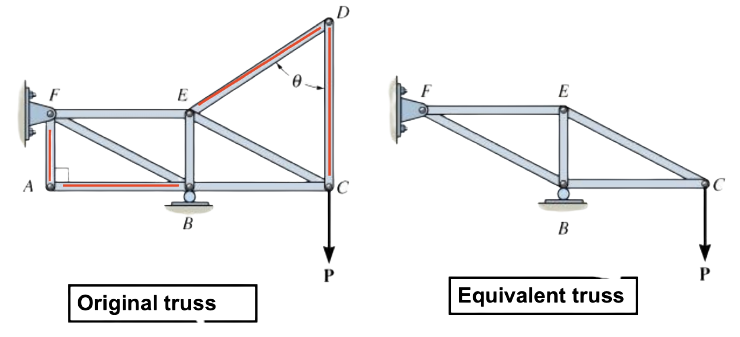
\includegraphics[width=0.45\textwidth]{./img/zero2.jpg}
        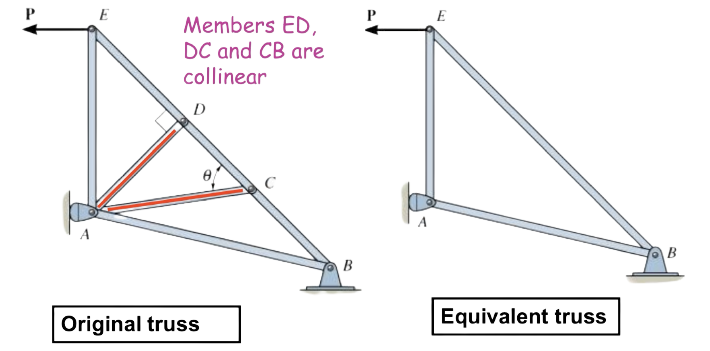
\includegraphics[width=0.45\textwidth]{./img/zero3.jpg}
    \end{center}
\end{theorem}

\subsection{Statically determinate trusses}
To construct an \emph{internally} statically determinate truss, we begin with a triangular pin-jointed truss and then successively adding two new members with a new joint.

We say the truss is only \emph{internally} statically determinate because the external reactions are not yet known.

\subsection{Truss analysis}
When we analyze a truss, we assume that forces are only applied at joints.
\begin{knBox}
    {Internal vs. External forces}
    \begin{itemize}
        \item Forces acting on the members $\to$ \textbf{Internal forces}
        \item Forces acting on joints $\to$ \textbf{External forces}
    \end{itemize}
\end{knBox}
\begin{definition}
    {Sign convention of analysis}
    As we focus on the analysis of \textbf{internal forces acting on joints}, we always draw:
    \begin{itemize}
        \item Tension forces $\to$ \textbf{pointing away} from the joint $\{\leftarrow\circ\boxed{\rightarrow\ T\ \leftarrow}\circ\rightarrow\}$
        \item Compression forces $\to$ \textbf{pointing towards} the joint $\{\rightarrow\circ\boxed{\leftarrow\ C\ \rightarrow}\circ\leftarrow\}$
    \end{itemize}
    During analysis, we always draw forces \textbf{pointing towards} the joint $\{\rightarrow\circ\leftarrow\}$, which means we treat \textbf{compression as positive}.

    We also treat \textbf{downward forces as positive} $\{+\downarrow\}$.
\end{definition}
\subsection{Equilibrium sections}
If we cut out any section of an equilibrium system, the cut will be in equilibrium. That is, the \textbf{external forces} are balanced by \textbf{internal forces}.

Therefore, to solve for the forces in a system, we simply cut out a section that we deem solvable (by practice!) and draw it's FBD. The forces includes \emph{all external forces in the cut} as well as the \emph{interal forces of the cut members}.

Note that to solve for a joint, the number of unknowns must be equal to the number of equations of equilibrium.

\subsection{Cable anaylsis}
\begin{definition}
    {Cable forces}
    Cables are \textbf{always in tension}. The tension force is always in the direction of the cable.
\end{definition}
Some characteristics of cable structures:
\begin{itemize}
    \item Supports are always 2 inverted pinned supports
    \item Applied forces all point downwards due to gravity
    \item Horizontal reaction forces at supports are equal in magnitude
\end{itemize}